\documentclass[aspectratio=169]{beamer}

\usetheme{Boadilla}
\usefonttheme{professionalfonts}
\setbeamertemplate{navigation symbols}{}
\setbeamertemplate{itemize items}[circle]
\setbeamertemplate{enumerate items}[default]
\setbeamertemplate{headline}{}

\usepackage[utf8]{inputenc}
\usepackage[T1]{fontenc}
\usepackage{lmodern}
\usepackage{amsmath}
\usepackage{booktabs}
\usepackage{tabularx}
\usepackage{array}
\usepackage{hyperref}
\usepackage[strings]{underscore}
\usepackage{listings}
\usepackage{tikz}
\usetikzlibrary{arrows.meta,positioning,fit,calc,shapes.geometric}
\usepackage{xcolor}

\definecolor{courseblue}{HTML}{12355B}
\definecolor{coursegold}{HTML}{C98A2E}
\definecolor{courseice}{HTML}{EEF3F8}
\definecolor{coursegreen}{HTML}{2F6B4F}
\definecolor{coursegray}{HTML}{4B5563}
\definecolor{codebg}{HTML}{F7F9FC}
\definecolor{codecomment}{HTML}{5E6C84}
\definecolor{codestring}{HTML}{0B6E4F}

\setbeamercolor{palette primary}{bg=courseblue,fg=white}
\setbeamercolor{palette secondary}{bg=coursegold,fg=white}
\setbeamercolor{palette tertiary}{bg=courseblue,fg=white}
\setbeamercolor{palette quaternary}{bg=coursegold,fg=white}
\setbeamercolor{structure}{fg=courseblue}
\setbeamercolor{frametitle}{bg=courseice,fg=courseblue}
\setbeamercolor{title}{fg=courseblue}
\setbeamercolor{block title}{bg=courseblue,fg=white}
\setbeamercolor{block body}{bg=courseice,fg=black}
\setbeamercolor{normal text}{fg=black,bg=white}
\setbeamercolor{alerted text}{fg=coursegold}

\setbeamerfont{footline}{size=\scriptsize}

\setbeamertemplate{footline}{
  \leavevmode
  \hbox{
    \begin{beamercolorbox}[wd=.33\paperwidth,ht=2.8ex,dp=1.2ex,leftskip=0.8em]{palette primary}%
      University of Trieste
    \end{beamercolorbox}%
    \begin{beamercolorbox}[wd=.49\paperwidth,ht=2.8ex,dp=1.2ex,center]{palette tertiary}%
      \coursename{} \textbar{} \coursecode
    \end{beamercolorbox}%
    \begin{beamercolorbox}[wd=.18\paperwidth,ht=2.8ex,dp=1.2ex,rightskip=0.8em plus1fil]{palette secondary}%
      \insertframenumber{} / \inserttotalframenumber
    \end{beamercolorbox}%
  }
}

\hypersetup{
  colorlinks=true,
  linkcolor=courseblue,
  urlcolor=coursegreen
}

\lstdefinestyle{coursepython}{
  language=Python,
  basicstyle=\ttfamily\footnotesize,
  keywordstyle=\color{courseblue}\bfseries,
  commentstyle=\color{codecomment}\itshape,
  stringstyle=\color{codestring},
  showstringspaces=false,
  columns=fullflexible,
  keepspaces=true,
  frame=single,
  framerule=0.6pt,
  rulecolor=\color{courseblue},
  backgroundcolor=\color{codebg},
  xleftmargin=0.4em,
  xrightmargin=0.4em,
  aboveskip=0.4em,
  belowskip=0.2em
}

\newcommand{\coursename}{Data-driven Systems Engineering}
\newcommand{\coursecode}{440MI / 305SM}
\newcommand{\coursefooter}{}

\newcommand{\learninggoals}[1]{
  \begin{block}{Learning goals}
  #1
  \end{block}
}

\newcommand{\repoactivity}[1]{
  \begin{block}{Repo activity}
  #1
  \end{block}
}

\newcommand{\readinglist}[1]{
  \begin{block}{Papers and materials}
  {\footnotesize #1}
  \end{block}
}

\newcommand{\coursecontextframe}[5]{
  \begin{frame}{Course Map and Running Cases}
  \centering
  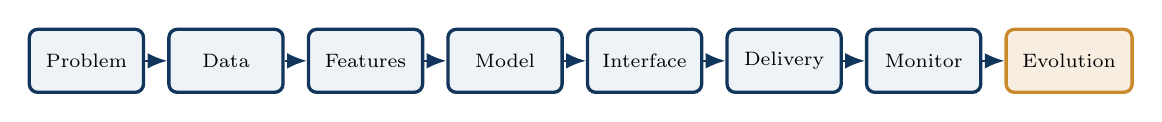
\begin{tikzpicture}[node distance=0.28cm]
  \node[flowbox, minimum width=1.45cm, minimum height=0.8cm] (problem) {\scriptsize Problem};
  \node[flowbox, minimum width=1.45cm, minimum height=0.8cm, right=of problem] (data) {\scriptsize Data};
  \node[flowbox, minimum width=1.45cm, minimum height=0.8cm, right=of data] (features) {\scriptsize Features};
  \node[flowbox, minimum width=1.45cm, minimum height=0.8cm, right=of features] (model) {\scriptsize Model};
  \node[flowbox, minimum width=1.45cm, minimum height=0.8cm, right=of model] (interface) {\scriptsize Interface};
  \node[flowbox, minimum width=1.45cm, minimum height=0.8cm, right=of interface] (delivery) {\scriptsize Delivery};
  \node[flowbox, minimum width=1.45cm, minimum height=0.8cm, right=of delivery] (monitor) {\scriptsize Monitor};
  \node[accentbox, minimum width=1.6cm, minimum height=0.8cm, right=of monitor] (evolution) {\scriptsize Evolution};
  \foreach \a/\b in {problem/data,data/features,features/model,model/interface,interface/delivery,delivery/monitor,monitor/evolution} {
    \draw[arrow] (\a) -- (\b);
  }
  \end{tikzpicture}

  \vspace{0.5em}
  \begin{block}{Today in the course}
  \textbf{Focus:} #1

  \textbf{Bridge:} #2
  \end{block}

  \begin{columns}[T]
  \column{0.48\textwidth}
  \begin{block}{Fraud case}
  {\footnotesize #3}
  \end{block}
  \column{0.48\textwidth}
  \begin{block}{Pasteurization case}
  {\footnotesize #4}
  \end{block}
  \end{columns}

  \vspace{0.3em}
  {\footnotesize \textbf{Course thread:} #5}
  \coursefooter
  \end{frame}
}

\newcommand{\classclosingframe}[4]{
  \begin{frame}{From This Class to the Next}
  \begin{block}{What stays with us}
  #1
  \end{block}

  \begin{columns}[T]
  \column{0.48\textwidth}
  \begin{block}{Project use}
  {\footnotesize #2}
  \end{block}
  \column{0.48\textwidth}
  \begin{block}{Next connection}
  {\footnotesize #3}
  \end{block}
  \end{columns}

  \vspace{0.3em}
  {\footnotesize \textbf{Course thread:} #4}
  \coursefooter
  \end{frame}
}

\tikzset{
  flowbox/.style={
    rounded corners=3pt,
    draw=courseblue,
    fill=courseice,
    very thick,
    minimum width=2.2cm,
    minimum height=0.9cm,
    align=center,
    font=\small
  },
  accentbox/.style={
    rounded corners=3pt,
    draw=coursegold,
    fill=coursegold!15,
    very thick,
    minimum width=2.2cm,
    minimum height=0.9cm,
    align=center,
    font=\small
  },
  arrow/.style={
    -{Latex[length=2.5mm,width=2mm]},
    thick,
    draw=courseblue
  }
}


\title{Class 18 Companion: The wine-wandb Project}
\subtitle{Dataset, structure, files, and libraries}
\author{\coursename}
\date{}

\newcommand{\hlcode}[1]{\colorbox{coursegold!35}{\bfseries #1}}

\begin{document}

\frame{\titlepage \coursefooter}

\begin{frame}{What this deck covers}
\begin{tabularx}{\textwidth}{>{\bfseries}l X}
1. The dataset & Origin, the 11 measurements, the target, and the preparation decisions. \\
\addlinespace[0.4em]
2. Project structure & Directories, root files, file types, and the role of each module. \\
\addlinespace[0.4em]
3. How a run works & Configuration, the data flow, and the reproducibility safeguards. \\
\addlinespace[0.4em]
4. Libraries & What each dependency does, with the calls the project actually uses. \\
\addlinespace[0.4em]
5. Running it & Tests, continuous integration, and the commands. \\
\bottomrule
\end{tabularx}
\vspace{0.8em}
\begin{block}{The project in one sentence}
\footnotesize A small, complete machine-learning project: a tracked baseline, a hyperparameter sweep, a versioned pipeline artifact, and a registry promotion, all for predicting red wine quality.
\end{block}
\coursefooter
\end{frame}

% ------------------------------------------------------------------ 1. Dataset
\begin{frame}{1. The dataset: Vinho Verde red wine}
\begin{itemize}
\item \textbf{Source:} UCI Machine Learning Repository, \emph{Wine Quality}; Cortez, Cerdeira, Almeida, Matos, Reis (2009), \emph{Decision Support Systems}, 47(4), 547--553.
\item \textbf{Content:} 1{,}599 red wines of the Portuguese Vinho Verde region, one row per wine.
\item \textbf{Inputs:} 11 physicochemical measurements obtained in the laboratory.
\item \textbf{Target:} \texttt{quality}, a sensory score from 0 to 10 given by wine experts (observed values: 3 to 8).
\item \textbf{Format:} one CSV file, \textbf{semicolon-separated}; 12 columns, no missing values.
\end{itemize}
\vspace{0.3em}
\begin{block}{Two caveats worth discussing}
\footnotesize
\textbf{Duplicates:} 240 rows are exact duplicates of another row. Copies that fall in both the training and the test split make the test score optimistic.
\textbf{Subjectivity:} the target is an expert opinion, not a measurement; part of the error is irreducible.
\end{block}
\coursefooter
\end{frame}

\begin{frame}{The 11 input features}
\begingroup\footnotesize
\begin{tabularx}{\textwidth}{>{\ttfamily}l l X r}
\normalfont\bfseries Column & \bfseries Unit & \bfseries Meaning & \bfseries Median \\
\toprule
fixed acidity & g/dm$^3$ & Non-volatile acids (mainly tartaric) & 7.9 \\
volatile acidity & g/dm$^3$ & Acetic acid; high values give a vinegar taste & 0.52 \\
citric acid & g/dm$^3$ & Adds freshness and flavor & 0.26 \\
residual sugar & g/dm$^3$ & Sugar left after fermentation & 2.2 \\
chlorides & g/dm$^3$ & Salt content & 0.079 \\
free sulfur dioxide & mg/dm$^3$ & Free SO$_2$ (preservative) & 14 \\
total sulfur dioxide & mg/dm$^3$ & Free plus bound SO$_2$ & 38 \\
density & g/cm$^3$ & Close to water; depends on alcohol and sugar & 0.997 \\
pH & --- & Acidity scale & 3.31 \\
sulphates & g/dm$^3$ & Potassium sulphate; an additive & 0.62 \\
alcohol & \% vol. & Alcohol content & 10.2 \\
\bottomrule
\end{tabularx}
\par\endgroup
\vspace{0.3em}
{\scriptsize Units and meanings follow the dataset documentation; medians were computed from the CSV.\par}
\coursefooter
\end{frame}

\begin{frame}{The target and the two tasks}
\begin{columns}[T]
\column{0.46\textwidth}
\centering
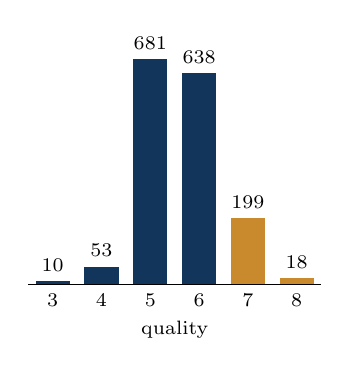
\begin{tikzpicture}[x=0.62cm, y=0.0042cm, font=\scriptsize]
\foreach \q/\n/\c in {3/10/courseblue, 4/53/courseblue, 5/681/courseblue, 6/638/courseblue, 7/199/coursegold, 8/18/coursegold}{
  \fill[\c] (\q-0.35,0) rectangle (\q+0.35,\n);
  \node[above] at (\q,\n) {\n};
  \node[below] at (\q,0) {\q};
}
\draw (2.5,0) -- (8.5,0);
\node[below=0.35cm] at (5.5,0) {quality};
\end{tikzpicture}

{\scriptsize Number of wines per quality score.\par}
\column{0.52\textwidth}
\begin{block}{Task 1: regression}
\footnotesize Predict \texttt{quality} itself. Metric: $R^2$ (and MAE, RMSE). Used by the tracked baseline and the sweep.
\end{block}
\begin{block}{Task 2: premium classification}
\footnotesize Predict \texttt{quality} $\ge 7$: 217 wines (13.6\%). Metrics: precision, recall, F1, AUC. Used by the evaluation slides.
\end{block}
\end{columns}
\vspace{0.3em}
\begin{itemize}\footnotesize
\item Strongest linear association with quality (Pearson): alcohol $+0.48$, volatile acidity $-0.39$, sulphates $+0.25$, citric acid $+0.23$.
\item Quality 3 and 8 are rare (10 and 18 wines); this is one reason the regression split is not stratified.
\end{itemize}
\coursefooter
\end{frame}

\begin{frame}{One dataset, two tasks, tracked the same way}
\begingroup\footnotesize
\begin{tabularx}{\textwidth}{>{\bfseries}l X X}
 & \textbf{\color{courseblue}Task 1: regression} & \textbf{\color{coursegold}Task 2: premium classification} \\
\toprule
Question & What is the quality score? & Is the wine premium (quality $\ge 7$)? \\
\addlinespace[0.2em]
Target & \texttt{quality}, 3 to 8 & 217 of 1{,}599 wines (13.6\%) \\
\addlinespace[0.2em]
Model & \texttt{GradientBoostingRegressor} & \texttt{RandomForestClassifier}, 300 trees \\
\addlinespace[0.2em]
Cross-validation & \texttt{KFold}, 5 folds & \texttt{StratifiedKFold}, 5 folds \\
\addlinespace[0.2em]
Selection metric & Cross-validated $R^2$ & Cross-validated F1-score \\
\addlinespace[0.2em]
Decision rule & None: the output is a number & The predicted class (\texttt{predict}) \\
\addlinespace[0.2em]
Tracked run & \texttt{train.py}, \texttt{sweep.py} & \texttt{train\_classifier.py} \\
\addlinespace[0.2em]
Artifact & \texttt{wine-pipeline}: \texttt{pipeline.joblib} & \texttt{wine-premium}: \texttt{pipeline.joblib} \\
\addlinespace[0.2em]
Used in class for & Tracking, sweeps, registry & Evaluation, decision-support example \\
\bottomrule
\end{tabularx}
\par\endgroup
\vspace{0.4em}
\begin{block}{Why two tasks?}
\footnotesize The same data answers two different questions. The choice of target space (a number or a class) changes the model and the metrics, and whether the output is already the answer or a class to act on.
\end{block}
\coursefooter
\end{frame}

\begin{frame}{Data preparation decisions and their reasons}
\begingroup\footnotesize
\begin{tabularx}{\textwidth}{>{\bfseries}p{3.2cm} X}
Decision & Reason \\
\toprule
Read with \texttt{sep=";"} & The UCI file uses semicolons, not commas. \\
\addlinespace[0.3em]
Fixed 75/25 split, seed 42 & 1{,}199 training and 400 test wines; the same partition for every run, so scores are comparable. \\
\addlinespace[0.3em]
Test split read only by \texttt{evaluate.py} and \texttt{figures.py} & Model selection uses cross-validation on the training split; the test split is evidence, not a tuning tool. \\
\addlinespace[0.3em]
\texttt{StandardScaler} inside the pipeline & Fitted on the training folds only, so no preprocessing leakage. Gradient boosting does not need scaling; it is kept to show the pattern and to allow scale-sensitive models. \\
\addlinespace[0.3em]
SHA-256 of the CSV logged per run & Identifies the exact dataset version used by each run. \\
\addlinespace[0.3em]
CSV not committed to Git & Downloaded on demand from the UCI repository; avoids redistributing the file and keeps the repository small. \\
\bottomrule
\end{tabularx}
\par\endgroup
\coursefooter
\end{frame}

% ------------------------------------------------------------------ 2. Structure
\begin{frame}[fragile]{2. Project structure}
\begin{lstlisting}[language={}, basicstyle=\ttfamily\footnotesize, frame=single, rulecolor=\color{courseblue}, backgroundcolor=\color{codebg}, columns=fixed, keepspaces=true, xleftmargin=0.4em, xrightmargin=0.4em]
wine-wandb/
|-- configs/                 baseline, sweep, classifier (YAML)
|-- src/wine_wandb/          the installable package
|   |-- data.py              download, checksum, load, split
|   |-- pipeline.py          task 1: scaler + gradient boosting
|   |-- premium.py           task 2: label, classifier, metrics
|   |-- train.py             task 1: tracked run + artifact
|   |-- train_classifier.py  task 2: tracked run + artifact
|   |-- sweep.py             W&B grid search (task 1)
|   |-- evaluate.py          test split, once (both tasks)
|   |-- register.py          link to the Registry
|   `-- figures.py           figures for the slides
|-- tests/                   pytest
|-- data/                    CSV downloaded here (not versioned)
|-- notebooks/               exploration only
|-- .github/workflows/       continuous integration
`-- README.md  requirements.txt  pyproject.toml  Makefile  .gitignore
\end{lstlisting}
\coursefooter
\end{frame}

\begin{frame}{Why each directory exists}
\begingroup\footnotesize
\begin{tabularx}{\textwidth}{>{\ttfamily}l X X}
\normalfont\bfseries Directory & \bfseries Contains & \bfseries Why it is separate \\
\toprule
configs/ & Seed, split, CV folds, default and swept hyperparameters (YAML) & Experiments change without touching code; a diff of a config is a diff of an experiment. \\
\addlinespace[0.3em]
src/wine\_wandb/ & Importable Python modules & A package can be tested and reused; each module has one responsibility. The \texttt{src} layout prevents importing uninstalled code by accident. \\
\addlinespace[0.3em]
tests/ & Unit and smoke tests & Fast checks that run in CI without data or an account. \\
\addlinespace[0.3em]
data/ & The downloaded CSV & Raw data stays outside the code, and outside Git. \\
\addlinespace[0.3em]
notebooks/ & Exploratory notebooks & Exploration is allowed, but the reproducible logic lives in \texttt{src/}. \\
\addlinespace[0.3em]
.github/workflows/ & CI definition & Every push runs the tests. \\
\bottomrule
\end{tabularx}
\par\endgroup
\vspace{0.3em}
{\scriptsize Generated locally and ignored by Git: \texttt{wandb/} (run logs), \texttt{artifacts/} (downloaded artifacts), \texttt{reports/} (figures and JSON).\par}
\coursefooter
\end{frame}

\begin{frame}{Root files}
\begingroup\footnotesize
\begin{tabularx}{\textwidth}{>{\ttfamily}l l X}
\normalfont\bfseries File & \bfseries Type & \bfseries Purpose \\
\toprule
README.md & Markdown & Overview, the two tasks, quick start, and the checkpoints. \\
\addlinespace[0.3em]
requirements.txt & Plain text & Runtime and test dependencies, each with a minimum version. \\
\addlinespace[0.3em]
pyproject.toml & TOML & Package metadata (name, version, Python $\ge 3.10$), the \texttt{src} layout, and the pytest settings. \\
\addlinespace[0.3em]
Makefile & Make & Short commands: \texttt{install}, \texttt{data}, \texttt{train}, \texttt{train-classifier}, \texttt{sweep}, \texttt{evaluate}, \texttt{evaluate-premium}, \texttt{figures}, \texttt{test}. \\
\addlinespace[0.3em]
.gitignore & Plain text & Keeps the CSV, \texttt{wandb/}, \texttt{artifacts/}, \texttt{reports/}, and environments out of Git. \\
\addlinespace[0.3em]
ci.yml & YAML & GitHub Actions: install, then run pytest with \texttt{WANDB\_MODE=disabled}. \\
\bottomrule
\end{tabularx}
\par\endgroup
\coursefooter
\end{frame}

\begin{frame}{File types in the project}
\begingroup\footnotesize
\begin{tabularx}{\textwidth}{>{\ttfamily}l l X}
\normalfont\bfseries Extension & \bfseries Format & \bfseries Role \\
\toprule
.py & Python source & Package modules and tests. \\
\addlinespace[0.25em]
.yaml / .yml & YAML & Experiment configuration and the CI workflow; human-readable and diff-friendly. \\
\addlinespace[0.25em]
.csv & Delimited text & The dataset (semicolon-separated); downloaded, never committed. \\
\addlinespace[0.25em]
.joblib & Binary (pickle-based) & The serialized \texttt{Pipeline}; stored as a W\&B artifact. Load only files you trust. \\
\addlinespace[0.25em]
.json & JSON & \texttt{reports/results.json}: the measured numbers behind the slides. \\
\addlinespace[0.25em]
.pdf & Vector graphics & Figures generated by \texttt{figures.py}. \\
\addlinespace[0.25em]
.md / .toml / .txt & Text & Documentation, packaging metadata, and dependency list. \\
\addlinespace[0.25em]
.gitkeep & Empty file & Keeps an otherwise empty directory (\texttt{data/}, \texttt{notebooks/}) in Git. \\
\bottomrule
\end{tabularx}
\par\endgroup
\coursefooter
\end{frame}

\begin{frame}{The package: one responsibility per module}
\begingroup\scriptsize
\begin{tabularx}{\textwidth}{>{\ttfamily}l >{\raggedright\arraybackslash}X >{\raggedright\arraybackslash}X}
\normalfont\bfseries Module & \bfseries Responsibility & \bfseries Main output \\
\toprule
data.py & \texttt{download}, \texttt{sha256}, \texttt{load}, \texttt{split} & DataFrame; train and test partitions \\
\addlinespace[0.1em]
pipeline.py & Task 1: scaler + \texttt{GradientBoostingRegressor}; rejects unknown hyperparameters & An unfitted \texttt{Pipeline} \\
\addlinespace[0.1em]
premium.py & Task 2: label (quality $\ge 7$), classifier pipeline, classification metrics & Pipeline; metrics \\
\addlinespace[0.1em]
train.py & Task 1 run: CV score, timing, final fit & \texttt{wine-pipeline} artifact \\
\addlinespace[0.1em]
train\_classifier.py & Task 2 run: cross-validated F1, precision, recall, ROC-AUC; final fit & \texttt{wine-premium} artifact \\
\addlinespace[0.1em]
sweep.py & Creates a sweep from \texttt{sweep.yaml}; the agent calls \texttt{train.run} & 81 runs \\
\addlinespace[0.1em]
evaluate.py & Scores an artifact on the test split (\texttt{--task regression} or \texttt{premium}) & \texttt{test/*} metrics \\
\addlinespace[0.1em]
register.py & Links an artifact version to a Registry collection & Registry entry \\
\addlinespace[0.1em]
figures.py & Test metrics of the classifier; overview and confusion-matrix figures & \texttt{reports/} (JSON, PDF) \\
\bottomrule
\end{tabularx}
\par\endgroup
\coursefooter
\end{frame}

\begin{frame}{Data flow: two tasks, one pattern}
\centering
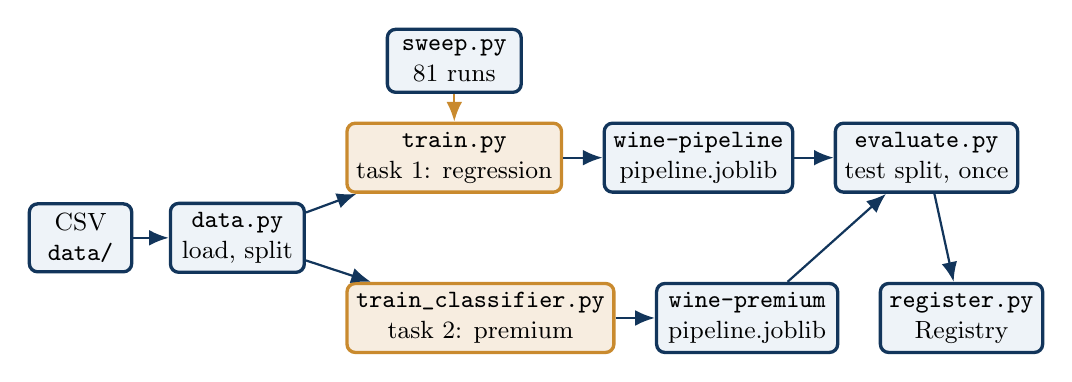
\begin{tikzpicture}[node distance=0.4cm, font=\scriptsize]
\node[flowbox, minimum width=1.3cm, minimum height=0.8cm] (csv) {CSV\\\texttt{data/}};
\node[flowbox, minimum width=1.7cm, minimum height=0.8cm, right=0.45cm of csv] (data) {\texttt{data.py}\\load, split};
\node[accentbox, minimum width=2.3cm, minimum height=0.8cm, above right=0.1cm and 0.5cm of data] (t1) {\texttt{train.py}\\task 1: regression};
\node[accentbox, minimum width=2.3cm, minimum height=0.8cm, below right=0.1cm and 0.5cm of data] (t2) {\texttt{train\_classifier.py}\\task 2: premium};
\node[flowbox, minimum width=2.3cm, minimum height=0.8cm, right=0.5cm of t1] (a1) {\texttt{wine-pipeline}\\pipeline.joblib};
\node[flowbox, minimum width=2.3cm, minimum height=0.8cm, right=0.5cm of t2] (a2) {\texttt{wine-premium}\\pipeline.joblib};
\node[flowbox, minimum width=1.8cm, minimum height=0.8cm, right=0.5cm of a1] (ev) {\texttt{evaluate.py}\\test split, once};
\node[flowbox, minimum width=1.8cm, minimum height=0.8cm, right=0.5cm of a2] (reg) {\texttt{register.py}\\Registry};
\node[flowbox, minimum width=1.7cm, minimum height=0.8cm, above=0.35cm of t1] (sw) {\texttt{sweep.py}\\81 runs};
\draw[arrow] (csv) -- (data);
\draw[arrow] (data) -- (t1); \draw[arrow] (data) -- (t2);
\draw[arrow] (t1) -- (a1); \draw[arrow] (t2) -- (a2);
\draw[arrow] (a1) -- (ev); \draw[arrow] (a2) -- (ev); \draw[arrow] (ev) -- (reg);
\draw[arrow, dashed, coursegold] (sw) -- (t1);
\end{tikzpicture}
\vspace{0.6em}
\begin{itemize}\footnotesize
\item Both runs log to W\&B and produce a versioned pipeline artifact; the premium classifier uses its predicted class as the decision.
\item Selection happens before \texttt{evaluate.py}: the test split never influences which artifact is chosen.
\end{itemize}
\coursefooter
\end{frame}

% ------------------------------------------------------------------ 3. A run
\begin{frame}[fragile]{3. Configuration: baseline and sweep}
\begin{columns}[T]
\column{0.46\textwidth}
{\footnotesize \texttt{configs/baseline.yaml}}
\begin{lstlisting}[language={}, basicstyle=\ttfamily\scriptsize, frame=single, rulecolor=\color{courseblue}, backgroundcolor=\color{codebg}, columns=fixed]
project: wine-quality
seed: 42
test_size: 0.25
cv_folds: 5
n_estimators: 100
max_depth: 3
learning_rate: 0.1
min_samples_split: 2
\end{lstlisting}
\column{0.52\textwidth}
{\footnotesize \texttt{configs/sweep.yaml}}
\begin{lstlisting}[language={}, basicstyle=\ttfamily\scriptsize, frame=single, rulecolor=\color{courseblue}, backgroundcolor=\color{codebg}, columns=fixed]
method: grid
metric:
  name: cv/r2_mean
  goal: maximize
parameters:
  n_estimators:
    values: [100, 200, 300]
  max_depth:
    values: [3, 5, 7]
  learning_rate:
    values: [0.05, 0.1, 0.2]
  min_samples_split:
    values: [2, 5, 10]
\end{lstlisting}
\end{columns}
\vspace{0.2em}
\begin{itemize}\footnotesize
\item The baseline gives the defaults; during a sweep, W\&B overrides the four hyperparameters and everything else (seed, split, folds) stays fixed.
\item The sweep metric is the cross-validated $R^2$ on the training split, never the test split. Task 2 has its own \texttt{classifier.yaml} (seed, split, folds, number of trees).
\end{itemize}
\coursefooter
\end{frame}

\begin{frame}{Anatomy of one run (\texttt{train.run})}
\begin{enumerate}\footnotesize
\item Read the YAML defaults and download the CSV if it is missing.
\item \texttt{wandb.init(config=defaults)}: open the run; a sweep agent overrides the swept values.
\item Log the dataset SHA-256 in the run configuration.
\item Load the data and split it with the configured seed; keep only the training partition.
\item Build the pipeline from the four hyperparameters.
\item 5-fold \texttt{KFold} (shuffled, seeded) with \texttt{cross\_val\_score}, scoring $R^2$; log \texttt{cv/r2\_mean}, \texttt{cv/r2\_std}, and \texttt{cv/seconds}.
\item Refit the pipeline on the whole training split, save it with \texttt{joblib}, and log it as the \texttt{wine-pipeline} artifact together with its hyperparameters and CV score as metadata.
\end{enumerate}
\vspace{0.4em}
\begin{block}{Why the refit?}
\footnotesize Cross-validation estimates quality but leaves no model behind. The refit produces the single object that can be evaluated, registered, and served.
\end{block}
\coursefooter
\end{frame}

\begin{frame}{Anatomy of the classifier run (\texttt{train\_classifier.run})}
\begin{enumerate}\footnotesize
\item Same start as task 1: YAML defaults, \texttt{wandb.init} with \texttt{job\_type="train-classifier"}, and the dataset SHA-256 logged in the configuration.
\item Split with the same seed; turn \texttt{quality} into the premium label (\texttt{quality} $\ge 7$).
\item \texttt{cross\_validate} with \texttt{StratifiedKFold} (5 folds) and four scores: F1, precision, recall, and ROC-AUC; log their means, the F1 standard deviation, and the time.
\item Refit on the whole training split and log one artifact, \texttt{wine-premium}, with \texttt{pipeline.joblib}.
\end{enumerate}
\vspace{0.4em}
\begin{block}{Why stratified folds and F1?}
\footnotesize Premium wines are 13.6\% of the data: stratification keeps that share in every fold, and F1 (unlike accuracy) is not inflated by the majority class.
\end{block}
\coursefooter
\end{frame}

\begin{frame}{Reproducibility safeguards}
\begingroup\footnotesize
\begin{tabularx}{\textwidth}{>{\bfseries}l X}
Risk & Safeguard in the project \\
\toprule
Different data & SHA-256 of the CSV logged in every run configuration. \\
\addlinespace[0.3em]
Different code & W\&B records the Git commit of the repository where the script runs. \\
\addlinespace[0.3em]
Different randomness & One seed for the split, the CV folds, and the model. \\
\addlinespace[0.3em]
Preprocessing mismatch & Scaler and model travel together in one serialized \texttt{Pipeline}. \\
\addlinespace[0.3em]
Preprocessing leakage & The scaler is refitted inside each training fold. \\
\addlinespace[0.3em]
Test-set leakage & Only \texttt{evaluate.py} and \texttt{figures.py} read the test split; selection uses CV. \\
\addlinespace[0.3em]
Silent regressions & Unit and smoke tests in CI; unknown hyperparameters raise an error. \\
\bottomrule
\end{tabularx}
\par\endgroup
\coursefooter
\end{frame}

% ------------------------------------------------------------------ 4. Libraries
\begin{frame}{4. Libraries and their roles}
\begingroup\footnotesize
\begin{tabularx}{\textwidth}{>{\bfseries}l l X}
Library & Minimum & Role in the project \\
\toprule
scikit-learn & 1.4 & Pipeline, preprocessing, models, cross-validation, and metrics. \\
\addlinespace[0.25em]
pandas & 2.1 & Reads the CSV into a DataFrame; separates features and target. \\
\addlinespace[0.25em]
NumPy & 1.26 & Numerical arrays: means and standard deviations of the CV scores. \\
\addlinespace[0.25em]
joblib & 1.3 & Serializes the fitted pipeline to \texttt{pipeline.joblib}. \\
\addlinespace[0.25em]
PyYAML & 6.0 & Reads the configuration files. \\
\addlinespace[0.25em]
Matplotlib & 3.8 & Figures for the slides (non-interactive \texttt{Agg} backend). \\
\addlinespace[0.25em]
wandb & 0.17 & Experiment tracking, sweeps, artifacts, and the Registry. \\
\addlinespace[0.25em]
pytest & 8.0 & Test runner. \\
\bottomrule
\end{tabularx}
\par\endgroup
\vspace{0.3em}
{\scriptsize Standard library: \texttt{argparse} (command lines), \texttt{hashlib} (SHA-256), \texttt{urllib.request} (download), \texttt{pathlib}, \texttt{json}, \texttt{tempfile}, and \texttt{time}.\par}
\coursefooter
\end{frame}

\begin{frame}{scikit-learn: the parts the project uses}
\begingroup\footnotesize
\begin{tabularx}{\textwidth}{>{\ttfamily}l X}
\normalfont\bfseries Component & \bfseries Use \\
\toprule
Pipeline & Chains \texttt{StandardScaler} and the model into one estimator with \texttt{fit} and \texttt{predict}. \\
\addlinespace[0.25em]
StandardScaler & Centers and scales each feature; parameters learned on the training data only. \\
\addlinespace[0.25em]
GradientBoostingRegressor & The regression model; tuned over \texttt{n\_estimators}, \texttt{max\_depth}, \texttt{learning\_rate}, \texttt{min\_samples\_split}. \\
\addlinespace[0.25em]
RandomForestClassifier & The premium-wine classifier (300 trees) in \texttt{premium.py}. \\
\addlinespace[0.25em]
train\_test\_split & The fixed, seeded 75/25 partition. \\
\addlinespace[0.25em]
KFold, StratifiedKFold & Folds for regression and for the imbalanced premium label. \\
\addlinespace[0.25em]
cross\_val\_score & Cross-validated $R^2$ for each configuration. \\
\addlinespace[0.25em]
cross\_validate & Several CV scores at once (F1, precision, recall, ROC-AUC) for the classifier. \\
\addlinespace[0.25em]
metrics & \texttt{r2\_score}, \texttt{mean\_absolute\_error}, \texttt{mean\_squared\_error}, \texttt{confusion\_matrix}, \texttt{f1\_score}, \texttt{roc\_auc\_score}, \texttt{average\_precision\_score}. \\
\bottomrule
\end{tabularx}
\par\endgroup
\coursefooter
\end{frame}

\begin{frame}{Weights \& Biases: the calls the project makes}
\begingroup\footnotesize
\begin{tabularx}{\textwidth}{>{\ttfamily}l X >{\ttfamily}l}
\normalfont\bfseries Call & \bfseries Purpose & \normalfont\bfseries Module \\
\toprule
wandb.init & Opens a run with its configuration; \texttt{job\_type} labels non-training runs. & train, evaluate, register \\
\addlinespace[0.12em]
run.config.update & Adds the dataset SHA-256 to the config. & train \\
\addlinespace[0.12em]
run.log & Sends metrics (\texttt{cv/*}, \texttt{test/*}). & train, evaluate \\
\addlinespace[0.12em]
wandb.Artifact & Creates a versioned \texttt{model} object with metadata. & train, train\_classifier \\
\addlinespace[0.12em]
artifact.add\_file & Attaches \texttt{pipeline.joblib}. & train, train\_classifier \\
\addlinespace[0.12em]
run.log\_artifact & Uploads it as a new version (\texttt{v0}, \texttt{v1}, \dots). & train, train\_classifier \\
\addlinespace[0.12em]
run.use\_artifact & Declares an input artifact (lineage); \texttt{.download()} fetches it. & evaluate, register \\
\addlinespace[0.12em]
run.link\_artifact & Publishes a version to a Registry collection. & register \\
\addlinespace[0.12em]
wandb.sweep, wandb.agent & Define the grid and execute the runs. & sweep \\
\bottomrule
\end{tabularx}
\par\endgroup
\coursefooter
\end{frame}

\begin{frame}{Supporting libraries in context}
\begin{columns}[T]
\column{0.48\textwidth}
\begin{block}{pandas and NumPy}
\footnotesize
\begin{itemize}\setlength{\itemsep}{1pt}
\item \texttt{pd.read\_csv(path, sep=";")} loads the data.
\item \texttt{df.drop(columns="quality")} gives the features; \texttt{df["quality"]} the target.
\item \texttt{np.mean}, \texttt{np.std} summarize the CV scores; \texttt{np.ndenumerate} labels the confusion matrix.
\end{itemize}
\end{block}
\begin{block}{joblib and PyYAML}
\footnotesize
\begin{itemize}\setlength{\itemsep}{1pt}
\item \texttt{joblib.dump} / \texttt{joblib.load} store and restore the pipeline.
\item \texttt{yaml.safe\_load} reads configs without executing arbitrary tags.
\end{itemize}
\end{block}
\column{0.48\textwidth}
\begin{block}{Matplotlib}
\footnotesize
\begin{itemize}\setlength{\itemsep}{1pt}
\item \texttt{matplotlib.use("Agg")} renders to files, so figures can be produced on a server or in CI.
\item Two PDF figures: dataset overview and confusion matrix.
\end{itemize}
\end{block}
\begin{block}{pytest}
\footnotesize
\begin{itemize}\setlength{\itemsep}{1pt}
\item Plain \texttt{assert} statements; fixtures build synthetic data.
\item \texttt{monkeypatch} sets \texttt{WANDB\_MODE=disabled} in the smoke test.
\end{itemize}
\end{block}
\end{columns}
\coursefooter
\end{frame}

% ------------------------------------------------------------------ 5. Running
\begin{frame}{5. Tests and continuous integration}
\begingroup\footnotesize
\begin{tabularx}{\textwidth}{>{\ttfamily}l c X}
\normalfont\bfseries File & \bfseries Tests & \bfseries What it checks \\
\toprule
test\_pipeline.py & 4 & Split is reproducible and sized correctly; the pipeline fits and predicts; it works inside cross-validation; unknown hyperparameters are rejected. \\
\addlinespace[0.2em]
test\_train\_smoke.py & 1 & \texttt{train.run} completes end to end on synthetic data, with W\&B disabled. \\
\addlinespace[0.2em]
test\_premium.py & 3 & The premium label; the counts and metrics of a small example (including ROC-AUC); the classifier pipeline fits and predicts. \\
\addlinespace[0.2em]
test\_train\_classifier\_smoke.py & 1 & \texttt{train\_classifier.run} completes end to end on synthetic data, with W\&B disabled. \\
\bottomrule
\end{tabularx}
\par\endgroup
\vspace{0.6em}
\begin{itemize}\footnotesize
\item The tests need neither the dataset download nor a W\&B account, so they run anywhere.
\item The GitHub Actions workflow installs the requirements and runs \texttt{pytest} on every push and pull request (Ubuntu, Python 3.11, \texttt{WANDB\_MODE=disabled}).
\item The sweep, evaluation, and registration need a W\&B account and are not part of CI. In total, 9 tests.
\end{itemize}
\coursefooter
\end{frame}

\begin{frame}[fragile]{Running the project}
\begin{lstlisting}[style=coursepython, language={}, columns=fixed]
python -m venv .venv && source .venv/bin/activate
make install
wandb login                    # once; not needed for the tests

make data                      # download the CSV
make train                     # task 1: baseline run
make sweep                     # task 1: 81 configurations
make train-classifier          # task 2: premium classifier
make evaluate ARTIFACT=wine-pipeline:v0         # test split, once
make evaluate-premium ARTIFACT=wine-premium:v0  # test split, once
make figures                   # dataset overview and confusion matrix
make test                      # no account required
\end{lstlisting}
\vspace{0.3em}
\begin{itemize}\footnotesize
\item Choose the artifact version by cross-validation; run the matching \texttt{evaluate} target once; then link it with \texttt{python -m wine\_wandb.register --artifact <name:version> --collection <registry path>}.
\end{itemize}
\coursefooter
\end{frame}

\begin{frame}{Summary}
\begin{block}{What the project demonstrates}
\footnotesize
\begin{itemize}\setlength{\itemsep}{1pt}
\item A \textbf{dataset} with known limits (subjective target, duplicates) and explicit preparation decisions.
\item A \textbf{structure} where configuration, code, tests, data, and generated files each have a place.
\item Two \textbf{tracked runs} (regression and premium classification) that record data, code, configuration, metrics, and a versioned pipeline.
\item \textbf{Libraries} chosen for one job each, with the minimum versions declared.
\end{itemize}
\end{block}
\vspace{0.3em}
\begin{block}{Connection to the next class}
\footnotesize The next class presents Streamlit and the dataset; the registered pipeline is the artifact an interface would load.
\end{block}
\coursefooter
\end{frame}

\end{document}
